\documentclass{article}
\usepackage[utf8]{inputenc}
\usepackage{graphicx}
\usepackage{amsmath}
\usepackage{listings}
\usepackage{geometry}
\geometry{a4paper, margin=1in}

\title{New York University \\ Tandon School of Engineering \\ Department of Computer Science and Engineering \\ Introduction to Operating Systems \\ Fall 2024 \\ Assignment 4 (10 points)}
\author{ }
\date{}

\begin{document}

\maketitle

\section*{Problem 1 (2 points)}

If you create a main() routine that calls fork() twice, followed by a call to execl(), i.e., if it includes the following code:

\begin{verbatim}
pid_t x=-11, y=-22;
x = fork();
if(x==0) y = fork();
if (y == 0) execl("/bin/ls", "ls", "-l", NULL);
\end{verbatim}

Assuming all fork() calls succeed, draw a process tree similar to that of Fig. 3.8 (page 116) in your textbook, clearly indicating the values of x and y for each process in the tree (i.e., whether 0, -11, -22, or larger than 0). Note that the process tree should only have one node for each process and thus the number of nodes should be equal to the number of processes. The process tree should be a snapshot just after all forks completed but before any process exits. Each line/arrow in the process tree diagram shall represent a creation of a process, or alternatively a parent/child relationship.  Consider the effect of `execl`.

(Insert process tree diagram here)


\section*{Problem 2 (4 points)}

Write a program that creates the process tree shown below:

\begin{center}
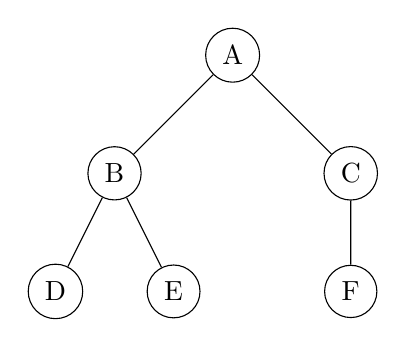
\begin{tikzpicture}[level distance=1.5cm,
  level 1/.style={sibling distance=3cm},
  level 2/.style={sibling distance=1.5cm}]
  \node[circle,draw] {A}
    child {node[circle,draw] {B}
      child {node[circle,draw] {D}}
      child {node[circle,draw] {E}}
    }
    child {node[circle,draw] {C}
      child {node[circle,draw] {F}}
    };
\end{tikzpicture}
\end{center}
Each node represents a process, and the edges represent the parent-child relationships.  Each process should print its own process ID.


\section*{Problem 3 (4 points)}

Write a program whose main routine obtains two parameters, n and m, from the user (passed to your program when invoked from the shell, n>0, m>0).  The parent process creates a child process. The child process calculates and prints the sum of integers from 1 to n. The parent process calculates and prints the product of integers from 1 to m (factorial). Do not use IPC in your solution (i.e., neither shared memory nor message passing).


\section*{Problem 4 (2 points)}

Explain the differences between fork(), vfork(), and clone() system calls in terms of their memory management and execution behavior.  Give examples where one might be preferred over the others.


\section*{Problem 5 (2 points)}

Draw a process state diagram showing the possible transitions between different process states (e.g., running, ready, blocked). Include at least five states and label the transitions with the events causing them.


\section*{Problem 6 (4 points)}

Write a C program that uses signals to handle the SIGINT (Ctrl+C) signal.  When SIGINT is received, the program should gracefully terminate after printing a message to the console, instead of abruptly exiting.  The program should also perform cleanup actions, such as closing any open files.


\section*{Problem 7 (2 points)}

Describe the zombie and orphan processes. Explain how these processes are created and how they can be avoided or handled properly.


\section*{What to hand in (using Brightspace):}

Please submit the following files individually:

\begin{enumerate}
    \item Source file(s) with appropriate comments. The naming should be similar to “lab\#\_\$.c” (\# is replaced with the assignment number and \$ with the question number within the assignment, e.g., \texttt{lab4\_b.c}, for lab 4, question b OR \texttt{lab5\_1a} for lab 5, question 1a).
    \item A single pdf file (for images + report/answers to short-answer questions), named “lab\#.pdf” (\# is replaced by the assignment number), containing:
    \begin{itemize}
        \item Screenshot(s) of your terminal window showing the current directory, the command used to compile your program, the command used to run your program, and the output of your program.
    \end{itemize}
    \item Your Makefile, if any. This is applicable only to kernel modules.
\end{enumerate}


\section*{RULES:}

\begin{itemize}
    \item You shall use kernel version 4.x.x or above. You shall not use kernel version 3.x.x.
    \item You may consult with other students about GENERAL concepts or methods but copying code (or code fragments) or algorithms is NOT ALLOWED and is considered cheating (whether copied from other students, the internet, or any other source).
    \item If you are having trouble, please ask your teaching assistant for help.
    \item You must submit your assignment prior to the deadline.
\end{itemize}


\end{document}